\chapter{Introducción}

El objetivo de este proyecto es evitar que un sistema \textit{blockchain} sea vulnerable a futuros ataques cuánticos. Para ello se ha implementado un algoritmo criptográfico resistente a ordenadores cuánticos, denominado UOV, para la firma de documentos, y posteriormente integrarlo en la \textit{blockchain} ARK.

\section{Motivación y contexto del proyecto}
\label{sec:intro:motivacion} %Esto se pone si queremos hacer referencia a esta sección

%En esta parte es importante clarificar las siguientes preguntas: 
%\begin{enumerate}
%\item ¿Cuál es el problema que pretendemos resolver con este proyecto? Debemos introducir un poco el contexto en el que aparece y describir bien en qué consiste dicho problema. 
%\item ¿Por qué es importante dicho problema? Hay que tratar de aportar datos y argumentos para indicar que el problema descrito es relevante en el contexto actual. 
%\end{enumerate}

La tecnología ha transformado nuestra sociedad en una sociedad digitalizada, donde actualmente, los dispositivos digitales comportan la mayor parte de nuestras actividades diarias en distintos ámbitos, como económicas, organizativas o sociales. En el proceso de digitalización de la sociedad podemos distinguir las siguientes cinco fases \cite{fases-digitalizacion}.\\

La primera fase o era del Internet, corresponde a mediados de los 90. En esta fase se comenzaron a crear páginas web para que los medios de comunicación y las empresas puedieran publicar y compartir información.

La segunda fase o era de las redes sociales, tuvo mayor auge a partir de 2005. Plataformas de bajo o ningún coste, se utilizaban en las empresas para poder llegar mejor a los clientes.

La tercera fase o era de la economía colaborativa, nació con la crisis de  2008 cuando las empresas tenían pocos recursos. Surgieron plataformas para conectar a las personas, y poder obtener lo que necesitasen unas de otras. Por ejemplo pagos online, ver recomendaciones y reseñas de un alojamiento o pedir un taxi. Además se da un gran paso ya que estas aplicaciones pasan de estar  alojadas en ordenadores a teléfonos inteligentes.

La cuarta fase o era del mundo autónomo, se ha desarrollado durante décadas. Se desarrollan tecnología con inteligencia artificial, es decir, que simulan la inteligencia de los humanos para poder resolver problemas más complejos.

Quinta fase o era del bienestar moderno, comienza con las pulseras inteligentes como \textit{Fitbit} o \textit{Fuelband} de Nike. Estas pulseras son el impulso de la tecnología para facilitar la vida de los clientes y poder integrar la tecnología en la vida de los mismos.\\

La digitalización debe de venir acompañada de mecanismos que aporten seguridad a los datos. Los pilares de la seguridad de la información son los conocidos como la tríada CIA (confidencialidad, integridad y  disponibilidad)\cite{servicios-seguridad}.\\

La \textbf{confidencialidad} es la propiedad que impide que la información pueda ser accesible por entidades no autorizadas. Un sistema garantiza la confidencialidad cuando un tercero entra en posesión de la información intercambiada entre el remitente y el destinatario, no es capaz de extraer ningún contenido legible. Para asegurar la confidencialidad se utilizan mecanismos de cifrado y ocultación de la comunicación.

La \textbf{integridad} busca mantener la exactitud de los datos, es decir, que no hayan sido modificados durante su envío. La integridad se obtiene adjuntando al mensaje otro conjunto de datos de comprobación de la integridad, un ejemplo es la firma digital.

La \textbf{disponibilidad} es la cualidad de la información de encontrarse a disposición de quienes deben acceder a ella, ya sean personas, procesos o aplicaciones, en el momentos que así lo quieran. Los mecanismos para asegurar la disponibilidad se implementan con la infraestructura tecnológica.\\

Además de estos tres pilares hay otro principio, la \textbf{autentificación}, que es la propiedad que permite identificar al generador de la información. Trata de comprobar si un mensaje enviado por un usuario, ha sido verdaderamente firmado por él mismo. Esto se consigue con el uso de cuentas de usuario y contraseñas de acceso.\\

Para garantizar estos servicios de seguridad se hace uso de protocolos de seguridad de la información entre los que se encuentra la criptografía, la lógica y la autenticación.\\

La criptografía se ocupa de cifrar ciertos mensaje con el fin de hacerlos ilegibles a receptores no autorizados, una vez que llega a su destino y sea descifrado, el receptor obtendrá el mensaje original \cite{criptografia}. Además dota de seguridad a las comunicaciones, a la información y a las entidades que se comunican.

Podemos diferenciar dos tipos de criptografía, la criptografía simétrica y la asimétrica. La criptografía simétrica utiliza la misma clave para cifrar y descrifrar un mensaje, esta clave la ha de conocer tanto el emisor como el receptor. Mientras que la asimétrica utiliza dos claves la pública y la privada.

En la criptografía asimétrica podemos diferenciar dos ramas, el cifrado de clave pública y las firmas digitales \cite{criptografia-asimetrica}. En el cifrado de clave pública, el emisor cifra el mensaje con la clave pública del destinatario y el receptor lo descifra con su propia clave privada. En las firmas digitales, el emisor firma el mensaje con su clave privada y el receptor puede verificar el mensaje con su propia clave pública, además cualquier manipulación del mensaje se refleja en su resumen o \textit{hash}.\\

Este tipo de criptografía basa su seguridad en la hipótesis de que no se pueden encontrar las claves por fuerza bruta con la tecnología existente en la actualidad. Los ataque de fuerza bruta tratan de recuperar las claves probando todas las posibles combinaciones hasta encontrar la que permite el acceso, a partir del algoritmo de cifrado y del texto cifrado con su original \cite{fuerza-bruta}. Para que la búsqueda tenga éxito se deberán de realizar $10^n-1$ operaciones donde $n$ es la longitud de la clave. 

Otro factor importante, en la seguridad, es si en la clave aparencen números, caracteres o la combinación de ambos, aumentando así el coste de encontrar las claves, llegando a alcanzar tiempos de cálculo logarítmicos, es decir, que podrían tardar siglos en encontrar una contraseña compleja pero también depende de la capacidad de operación del ordenador.\\

En este contexto, la aparición de la futura computación cuántica permitirá el cálculo de operaciones a una velocidad mucho mayor. En la gráfica \ref{fig:comp-clasica-cuantica} podemos observar la capacidad de cómputo del peor ordenador cuántico, con la línea continua, que sigue la gráfica de una función exponencial, frente a la capacidad del mejor ordenador clásico, la línea discontinua, que sigue una función lineal.

\begin{figure}[h]
	\centering
	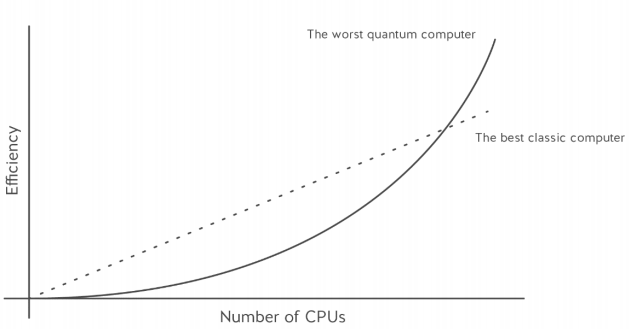
\includegraphics[width=0.8\textwidth]{figuras/comp_clasica_cuantica.png}
	\caption{Comparativa de la capacidad de cómputo de un ordenador clásico con un ordenador cuántico\cite{clasica-vs-cuantica}}
	\label{fig:comp-clasica-cuantica}
\end{figure}

La comparativa también nos muestra que para operaciones pequeñas como, por ejemplo, editar un documento de texto un ordenador cuántico sería probablemente ineficienciente. Por tanto lo mejor sería un ordenador híbrido, que mezclase computación clásica, para cálculos pequeños, y computación cuántica, para operaciones de mayor tamaño.\\

Cuando esté desarrollado el ordenador cuántico no serán válidos los actuales algoritmos criptográficos de clave pública, como \acrshort{rsa}, Diffie-Hellman y \mbox{\acrshort{ecdsa}}, ya que se basan en los problemas del logaritmo discreto y factorización de enteros, resolubles fácilmente por un ordenador cuántico. Las primeras ideas de la criptografía cuántica se tiene en los años 70, destacando los algoritmos de Shor y Grover.

Veamos la tabla comparativa \ref{table:security-level}, esta nos indica el tipo de algoritmo criptográfico, el algoritmo con la longitud de la clave y a continuación el nivel de seguridad tanto en un ordenador clásico como en uno cuántico. El nivel de seguridad de un algoritmo nos indica el número de operaciones necesarias para romper dicho algoritmo, por ejemplo, si tiene un nivel de seguridad $n$ entonces se requieren $2^n$ operaciones para romper el algoritmo \cite{security-level}. Observamos que hay una diferencia considerable en los niveles de seguridad de los algoritmo asimétricos, puesto que con un ordenador clásico al menos se necesitan $2^{112}$ operaciones mientras que con computación cuántica solo una. \\

\begin{table}[h]
	
	\label{table:security-level}
	\centering
	\resizebox{\linewidth}{!}{
	\begin{tabular}{c c c c c }
		\hline \\[-1.5ex]
		\thead{Tipo} & \thead{Algoritmo-Longitud clave} & \thead{Nivel seguridad\\ (ordenador clásico)} & \thead{Nivel seguridad\\ (ordenador cuántico)} & \thead{Ataque cuántico}\\ [1ex] 
		\hline\hline \\[-1.5ex]
		\multirow{4}{5em}{Asimétrico} & RSA-2048 & 112 & 0 & Algoritmo de Shor \\ [0.5ex]
		& RSA-3072 & 128 & 0 & Algoritmo de Shor \\ [0.5ex]
		& ECC-521 & 128 & 0 & Algoritmo de Shor \\ [0.5ex]
		& ECC-521 & 256 & 0 & Algoritmo de Shor \\ [0.5ex]
		\hline \\[-1.5ex]
		\multirow{2}{5em}{Simétrico} & AES-128 & 128 & 64 & Algoritmo de Grover \\ [0.5ex]
		& AES-256 & 256 & 128 & Algoritmo de Grover \\ [1ex]
		\hline
	\end{tabular}}
	\caption{Niveles de seguridad de ordenadores clásicos y cuánticos \cite{security-bit}}
\end{table}


En la actualidad, se están desarrollando muchos algoritmos para que sean resistentes a ataques de tipo cuántico, denominados algoritmos de criptografía postcuántica \cite{criptografia-postcuantica}. Estos ataques afectan principalmente a los algoritmos de clave pública o asimétrica, puesto que para la criptografía simétrica duplicar el tamaño de clave empleada es suficiente para hacerlos seguros y hacer inservible el algoritmo de Grover.\\

Por otro lado, también en la actualidad está siendo muy relevante la adopción de las \textit{blockchain} como tecnología para ofrecer diversos servicios. Las \textit{blockchain} o cadenas de bloques son listas de transacciones, denominadas bloques, firmadas y unidas con algoritmos criptográficos. Además cada bloque contiene el hash del bloque anterior, se explicará con más detalle en la sección \ref{sec:intro:blockchain}. 

Esta tecnología se ha integrado en diferentes áreas, donde resalta el uso en los servicios financieros o criptomonedas, que aumenta la eficiencia y disminuye los costes. Otro uso de las \textit{blockchain} es en las cadenas de suministro, algunos restaurantes, como Fogo de Ch\~{a}o \cite{Fogo-Chao}, están empezando a utilizar las \textit{blockchain} para poder rastrear el origen de sus alimentos hasta llegar al propio restaurante, una gran ventaja para encontrar fácilmente si hay algún producto contaminado o en mal estado. \\

Un ejemplo del uso de las \textit{blockchain} queda reflejado en este proyecto en el que se ha implementado un algoritmo resistente a ataques cuánticos, UOV \cite{algoritmo-UOV} y se ha adaptado a la \textit{blockchain} ARK \cite{ark} para que se utilice dicho algoritmo de firma.\\


\section{Objetivos del proyecto y logros conseguidos}
\label{sec:intro:objetivos}
El objetivo de este proyecto es modificar el algoritmo de firma y verificación de las transacciones de la \textit{blockchain} ARK, para hacerla resistente a ataques cuánticos.

\begin{itemize}
	\item Implementación del algoritmo UOV: Se ha implementado las funciones de generación de claves tanto públicas como privadas, la función de firma a partir de la clave privada y la función de verificación de la misma con la clave pública. Además ha sido necesario implementar la aritmética de cuerpo finito de $2^7$ elementos.
	\item Integrar el algoritmo UOV en la \textit{blockchain} ARK para comprobar su funcionamiento: Se ha modificado el algoritmo de firma dado en la \textit{blockchain} por el algoritmo UOV para aumentar la seguridad.

\end{itemize}


\section{Estructura de la memoria}
%Se describirán los capítulos que tiene la memoria, indicando qué contenidos habrá en cada uno de ellos, para permitir al lector situarse ante el documento. 

A continuación se muestran los capítulos que presenta la memoria junto con una breve descripción de lo que contiene cada uno.

\begin{enumerate}
	\item Introducción: Presenta la motivación del proyecto y el contexto en el que surge, además incluye una breve reseña introduciendo las dos tecnologías que se han utilizado computación cuántica y la \textit{blockchain}, aparte de la explicación matemática del algoritmo utilizado. En este capitulo también se encuentran los objetivos que se persiguen con este trabajo.
	\item Planificación y costes: Contiene el diagrama de Gantt con la defición de las entregas y seguimiento del proyecto, así como el presupuesto del proyecto.
	\item Análisis del problema: Descripción de las funcionalidades y requisitos, y análisis de los objetivos que se muestran en la sección \ref{sec:intro:objetivos}.
	\item Diseño: Se encuentra el diseño de la implementación del algoritmo UOV y el diseño del ecosistema ARK, donde se integrará el algoritmo de firma.
	\item Implementación: Contiene la explicación de la implementación del algoritmo UOV y la aritemética del cuerpo finito de $2^7$ elementos.
	\item Evaluación y pruebas: Ejemplo de la firma de una transacción en el sistema ARK.
	\item Conclusiones
\end{enumerate}

\section{Contenidos teóricos para la comprensión del proyecto}

En los siguientes apartados se explica los contenidos claves de este proyecto, que son la computación cuántica\ \ref{sec:intro:cc}, la tecnología \textit{blockchain}\ \ref{sec:intro:blockchain} y el algoritmo UOV\ \ref{sec:intro:UOV}.

\subsection{Computación cuántica}\label{sec:intro:cc}
%Poner un poco de historia ver 

%\url{https://es.wikipedia.org/wiki/Computaci%C3%B3n_cu%C3%A1ntica#Cronolog%C3%ADa}
%\url{http://openaccess.uoc.edu/webapps/o2/bitstream/10609/89026/6/alvaroreyesTFM1218memoria.pdf}

La computación cuántica constituye un nuevo paradigma de la informática basado en los principios de la teoría cuántica. Los ordenadores cuánticos 

La computación clásica funciona con bits cuyos valores pueden ser 0 o 1, mientras que la computación cuántica funciona con bit cuánticos o cúbits, una combinación de 0 y 1, pudiendo tomar ambos valores a la vez, esto se denomina la superposición cuántica de los estados \cite{computacion-cuantica-criptografia}, se explicará un poco más adelante.
La figura \ref{fig:bit-cubit} muestra

\begin{figure}[h]
	\centering
	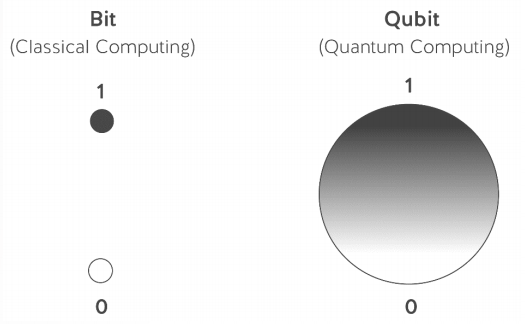
\includegraphics[width=0.8\textwidth]{figuras/bit_cubit.png}
	\caption{Comparativa de la capacidad de cómputo de un ordenador clásico con un ordenador cuántico\cite{clasica-vs-cuantica}}
	\label{fig:bit-cubit}
\end{figure}

El espacio de estados del cúbit se puede representar mediante un espacio vectorial complejo bidimensional, al no ser práctico se aprovecha el homeomorfismo entre la superficie de una esfera y el plano complejo cerrado con un punto en el infinito, dando lugar a lo que se conoce como la esfera de Bloch.  Una esfera de Bloch es una representación geométrica del espacio de estados puros de un sistema cuántico de dos niveles. Además se representa en el espacio $\mathds{R}^3$ por la esfera de radio unidad. Ver la imagen \ref{fig:esfera-bloch}.

\begin{figure}[h]
	\centering
	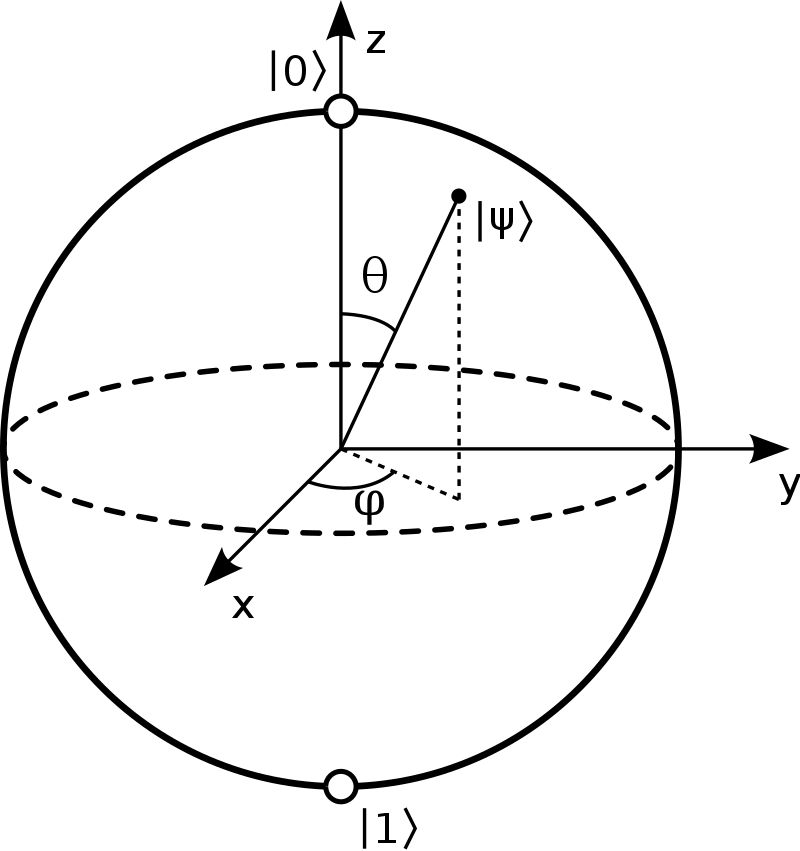
\includegraphics[width=0.4\textwidth]{figuras/esfera_bloch.png}
	\caption{Estructura cúbit, esfera de Bloch \cite{esfera-bloch}}
	\label{fig:esfera-bloch}
\end{figure}

La superposición cuántica aporta gran capacidad de procesamiento, lo que hace posible resolver de manera eficiente problemas de mayor complejidad como la factorización de enteros, el algoritmo discreto y la simulación cuántica, que a día de hoy con los ordenadores clásicos son difíciles de romper. 

Otro aspecto importante de la física cuántica relacionado con la superposición es el entrelazamiento de las partículas\cite{cumputacion-cuantica-clasica}. Esto es, si dos partículas en algún instante han interactuado retienen un tipo de conexión y pueden entrelazarse formando pares. Esto permite que aunque los cúbits estén separados interactúen entre sí. Con estos dos aspectos la capacidad de procesamiento aumenta considerablemente, cuántos más cúbits la capacidad de procesamiento aumenta considerablemente.


La evolución de la tecnología se ha basado principalmente en la reducción de los transistores para aumentar la velocidad, llegando a escalas de tan solo algunas decenas de nanómetros. Esto tiene un límite y es la eficiencia, puesto que al seguir disminuyendo el tamaño podrían dejar de funcionar correctamente. De ahí surge la necesidad de descubrir nuevas tecnologías, la computación cuántica \cite{computacion-cuantica-wiki}.

El estudio de las tecnologías cuánticas se inició en 1980, donde surgieron teorías con la posibilidad de realizar cálculos cuánticos. En la década de los 90 se empezó a poner en práctica algunas teoría, apareciendo los primeros algoritmos cuánticos, primeras aplicaciones cuánticas y las primera máquinas diseñadas para realizar cálculos cuánticos.\\

Google ha logrado aplicar una supercomputadores al mundo real, simulando con éxito una reacción quñimica simple. Marcando el camino hacia la química cuántica. Esto podría ayudar a los científicos a comprender mejor las reacciones moleculares, dando lugar a descubrimientos útiles como mejores baterías, nuevas formas de producir fertilizante y métodos para eliminar el dióxido de carbono del aire \cite{quimica-cuantica}.

\subsection{Blockchain}\label{sec:intro:blockchain}


\textit{Blockchain} es un sistemas de almacenamiento de información que se divide en bloque de datos enlazados mediante los hash. A cada bloque se le asocia un hash a partir del bloque anterior, creando una lista enlazada, la búsqueda de información no es muy óptima si hay un número elevado de bloques. Para la búsqueda eficiente en \textit{blockchain} se usan los árboles merkle.\\

Los datos que almacena cada bloque son transacciones válidas, información referente a ese bloque y la relación con el bloque anterior mediante el \textit{hash}, por tanto el bloque tiene un lugar específico dentro de la cadena. De esta forma si hay una alteración en un determinado bloque se verá reflejado en su \textit{hash} y en el de los bloques posteriores, haciendo que la información de la cadena no se pueda perder, modificar o eliminar.\\


Los árboles merkle \cite{arbol-merkle} son una estructura de datos en árbol en el que cada nodo que no es hoja está etiquetado con el \textit{hash} que surge de la combinación de los valores o etiquetas de sus nodos hijo. Esta estructura permite que aunque los datos estén separados puedan ser ligados a un único valor de \textit{hash}, el \textit{hash} del nodo raíz del árbol. El \textit{hash} de este nodo va firmado para asegurar la integridad y hacer que la verificación sea fiable. 

De esta forma se asegura que los datos son recibidos sin daños y sin ser alterados, además permite que los datos puedan ser entregados por partes, ya que un nodo puede obtener solo la cabecera de un bloque desde una fuente y otra pequeña parte del árbol desde otra fuente, y poder asegurar que los datos son correctos. Esto funciona porque si un usuario intenta hacer un cambio en una transacción falsa en la parte inferior del árbol en seguida se verá reflejado en la parte superior del árbol, es decir, en el nodo raíz. Esta propiedad se ve clara en la estructura del árbol Merkle \ref{fig:arbol-Merkle}, donde los \textit{hash} de los nodos superiores se calculan a partir de los \textit{hash} de los nodos hijos.\\

\begin{figure}[h]
	\centering
	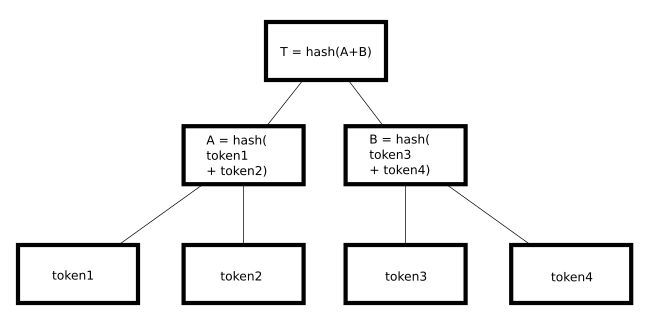
\includegraphics[width=0.8\textwidth]{figuras/arbol_merkle.png}
	\caption{Estructura de un árbol Merkle \cite{img-arbol-merkle}}
	\label{fig:arbol-Merkle}
\end{figure}

La idea de la tecnología \textit{blockchain} surge a comienzos de 1991 cuando los científicos Stuart Haber y W. Scott Stornetta introducen una solución computacional para la firma de documentos digitales y que no puedieran ser modificados con el tiempo. Usaron cadenas de bloque para almecenar los documentos con sello de tiempo y en 1992 se incorporaron los árboles Merkle, que podían recopilar varios documentos en un bloque haciendo el diseño más eficiente. Sin embargo, esta tecnología no se utilizó y la patente caducó en 2004 \cite{historia1-block}.

En 1998, Nick Szabo trabaja en una moneda digital descentralizada, ``bit gold''. Dos años después Stefan Konst publica su teoría sobre la seguridad criptográfica en las cadenas de bloques junto con algunas ideas de implementación \cite{historia2-block}.

En 2004, el informático y criptógrafo Harold Thomas Finney introdujo el sistema RPoW (prueba de trabajo reutilizable). El sistema se basa en \textit{HashCash} pero los token de prueba no están ligados a una aplicación sino que pueden ser gastados libremente como una moneda. Los clientes pueden crear tokens e intercambiarlos sin necesidad de regenerarlos \cite{RPoW}. RPoW resolvió el problema del doble gasto registrando los tokens en un servidor fiable diseñado para permitir a los usuarios verificar su exactitud e integridad en tiempo real. Este sistema puede considerarse como un prototipo de las criptomonedas.

A finales de 2008, un grupo de desarrolladores bajo el nombre de Satoshi Nakamoto publican un documento técnico en que se establece un modelo para \textit{blockchain}. Está basado en el algoritmo RPoW pero en lugar de usar dicho hardware, se utiliza un protocolo descentralizado peer-to-peer para verificar y restrear las transacciones. En otras palablas los ``mineros'' extraen bitcoins para obtener una recompensa mediantes pruebas de trabajo y posteriormente los nodos los verifican. Bitcoin nació el 3 de enero de 2009 cuando Satoshi Nakamoto extrajo el primer bloque de bitcoin con una recompensa de 50 bitcoins. Y el 12 de enero de 2009 tuvo lugar la primera transacción entre Satoshi Nakamoto y Hal Finney que obtuvo 10 bitcoins.

A partir de 2014, se comienzan a explorar el potencial de las cadenas de bloque y a buscar otras aplicaciones fuera de su uso en las transacciones financieras.
Ethereum introduce programas informáticos que se ejecutan en la \textit{blockchain}, se pueden utilizar para realizar una transacción cumpliendo ciertas condiciones como los contratos inteligentes.

Un contrato inteligenete se tratan de contratos que tienen la capacidad de cumplirse de forma automática. Un contrato inteligente está constituido por un protocolo de códigos que permiten a un dispositivo ejecutar de forma automatizada las sentencias previamente programadas, prescindiendo de la intervención humana \cite{contrato-inteligente}.

Además de los contratos inteligentes, Ethereum tiene su propia criptomoneda llamada Ether, se puede transferir entre cuentas y se utiliza para pagar las tarifas por la ejecución de los contratos inteligentes.

Actualmente las \textit{blockchain} tiene otros usos más allá de las criptomonedas.\\


Las cadenas de bloques o \textit{blockchain} permiten verificar, validar, rastrear todo tipo de información, ya sean contratos inteligentes, transacciones financieras, certificados digitales o firmas \cite{blockchain}, siendo estas últimas el centro de este trabajo. También permiten impulsar modificaciones orientadas a crear soluciones más robustas, por ejemplo en centros de salud o notarías que se explicarán más adelante.\\

Las \textit{blockchain} son vulnerables a futuros ataques cuánticos ya que su única línea de defensa es el algoritmo de firma de los bloques. Aunque, actualmente las cadenas de bloques son seguras, puesto que un ordenador clásico no tiene la capacidad de cómputo necesaria para descifrar cada bloque, obtener la información y volver a firmar todos los bloques sin dejar huella. Por eso para hacer una \textit{blockchain} resistente es necesario tener un criptosistema que no se pueda romper con computación cuántica, como por ejemplo el algoritmo UOV, ver apartado \ref{sec:intro:UOV}. \\

Los tres pilares de la tecnología \textit{blockchain} son la descentralización, transparencia e inmutabilidad \cite{pilares-blockchain}.

Un sistema centralizado almacena todos los datos en una misma entidad y habría que interactuar con la misma para obtener la información necesaria. Un ejemplo de un sistema centralizado son los bancos que almacenan todo el dinero y la única forma de pagar a alguien es a través de un banco. Es similar a la arquitectura cliente-servidor donde los clientes se comunican entre ellos mediante el servidor. Pero tener un único sitio para almacenar todos los datos es vulnerable a los ataques, informáticos, por otra parte si el nodo central se corrompe o tiene una actualización, los datos será incorrectos o no se podrán acceder a ellos. De los contras de los sistemas centralizados surge la idea de los sistemas \textbf{descentralizados}, la información no la tiene un único nodo sino que todos los usuarios son dueños de la información. La principal ideología de las \textit{blockchain} es poder interactuar usuario con usuario sin tener que pasar por un tercero.

El concepto \textbf{transparencia} se refiere a la transparencia de los datos no de las identidades. Esto es la identidad de la persona se oculta a través de la criptografía y lo único que se ve es su dirección pública, pero podemos ver todas las transacciones que se han realizado en su dirección pública. En el historial de transacciones no vemos ``Antonio envió 1BTC'' sino que aparece ``\sloppy{1MF1bhsFLkBzzz9vpFYEmvwT2TbyCt7NZJ} envió un 1BTC''. Este nivel de transparencia nunca antes había existido en el sistema financiero, lo que exige más responsabilidad a las grandes empresas. De la misma forma podemos trasladar este concepto fuera del sistema financiero por ejemplo a las cadenas de suministro, y saber exactamente de donde provienen los alimentos de un restaurante.

La \textbf{inmutabilidad} en el contexto de las cadenas de bloques significa que una vez introducida una transacción en la \textit{blockchain} ya no se puede alterar. De esta forma aplicando esta tecnología a los bancos se evitarían casos de malversación de fondos. Esta propiedad se obtiene gracias a la función criptográfica \textit{hash}.

La función \textit{hash} es el resultado de aplicar una función que transforma un mensaje de longitud variable en uno de longitud fija. Esto es calcular el resto módulo $n$ con $n$ la longitud fija. Al aplicar la función hash a un fichero, si se modifica algún dato del mismo cambiará su hash y por tanto se sabrá si ha sido manipulado desde que se envió, consiguiendo la integridad del mensaje.

De la misma forma si hay un cambio en una de las transacciones de un bloque se reflejará en el \textit{hash} del bloque, afectado a todos los bloques anteriores. Así si el atacante quiere preservar la integridad deberá de modificar todos los bloques siendo una tarea imposible. De esta forma se obtiene la inmutabilidad de los datos.\\

Hoy en día, la tecnología \textit{blockchain} está ganando mucha atención, no limitandose solo al uso en las criptomonedas. Así las cadenas de bloques tienen diversas aplicaciones entre ellas se encuentra la salud o la firma de documentos en las notarías. En el primer caso, cada centro  de salud podría tener el historial médico de cualquier paciente, de una forma segura y evitando falsificaciones, estos historiales se encontrarían en nodos distribuidos de forma descentralizada así se obtendría un acceso rápido y seguro. El segundo caso será en el que nos centraremos a lo largo de este proyecto. Hoy día la firma de documentos o transacciones por parte de un usuario es un problema puesto que se pueden copiar con facilidad, pero con \textit{blockchain} no podrían ser falsificadas debido a la propiedad de validación y rastreo de los datos.\\


\subsection{Algoritmo UOV}\label{sec:intro:UOV}


\subsubsection{Cuerpos finitos} % revisar con javier
Se trabajará con el cuerpo finito de 128 elementos, $\GF(2^7)$, que es un cuerpo extendido de $\GF(2)$ que corresponde con el cociente 
\begin{equation}
\GF(128) = \frac{\GF(2)[x]}{\langle x^7 + x + 1 \rangle}
\end{equation}

Además el orden del cuerpo de las unidades es $127$, que es primo entonces todo elemento del cuerpo distinto de $1$ es un elemento primitivo, es decir, un generador.

La tabla \ref{tab:rel} muestra una representación de los elementos no nulos del cuerpo. En la implementación se ha utilizado la representación como cadena de bits, puesto que a la hora de trabajar es más fácil con una cadeba de bits que con los polinomios.

\begin{table}[h]
\caption{Representación de los elementos no nulos del cuerpo finito de $2^7$ elementos}
\label{tab:rel}
\begin{center}
\begin{tabular}{p{0.2\linewidth}p {0.2\linewidth}p{0.2\linewidth}}
	 \textbf{Polinomio} & \textbf{Bits} & \textbf{$\log_a$}\\
\toprule
	$1$ & [0, 0, 0, 0, 0, 0, 1] & 0\\
	$a$ & [0, 0, 0, 0, 0, 1, 0] & 1\\
	$a^2$ & [0, 0, 0, 0, 1, 0, 0] & 2\\
	\\
	$\vdots$ & $\vdots$ & $\vdots$\\
	\\
	$a^6 + a^5 + a^4 + 1$ & [1, 1, 1, 0, 0, 0, 1] & 124\\
	$a^6 + a^5 + 1$ & [1, 1, 0, 0, 0, 0, 1] & 125\\
	$a^6 + 1$ & [1, 0, 0, 0, 0, 0, 1] & 126\\
\bottomrule
\end{tabular}
\end{center}


\end{table}

La implementación del cuerpo finito de $2^7$ elementos no se ha realizado de forma genérica sino para que sea específica para el algoritmo UOV, de esta forma es mucho más sencillo implementar la aritmética del cuerpo. Para la suma en $\mathds{Z}_2$ sólo tenemos que fijarnos que es lo mismo que el operador lógico \textit{XOR}, mientras que para el producto, al encontrarmos en un cuerpo como un orden pequeño, se usarán unas tablas que contienen las correspondencias entre los elementos no nulos del cuerpo y sus logaritmos en base $a$, por lo que el producto se convierte en una suma módulo $127$.




\subsubsection{Parámetros y fórmula}
Para empezar indicamos los parámetros que serán de utilidad para entender el algoritmo.
\begin{itemize}
	\item r: Grado del cuerpo extendido, $\mathds{F}_2 \subset \mathds{F}_{2^r}$. % quitar el F_2
	\item $x$: Vector de $n$ componentes, denominando a las primeras $v$ componentes  $x_1, \dotsb, x_v$ vinagre y al resto aceites.
	
	\item m: Tamaño de la clave pública, además del número de variables de aceite.
	\item $v$: Número de variables vinagre.
	%\item $\mathcal{H}$: Función salida extensible se usa para crear el hash del mensaje y proviene de la clave pública.
	%\item $\mathcal{G}$: Función salida extensible se usa para la generación de la clave pública a partir de una semilla privada.
\end{itemize}

$\mathcal{P}: \mathds{F}_{2^r}^n \rightarrow \mathds{F}_{2^r}^m$, esta función se puede descomponer como $\mathcal{P} = \mathcal{F} \circ \mathcal{T}$, donde $\mathcal{T}: \mathds{F}_{2^r}^n \rightarrow \mathds{F}_{2^r}^n$ es invertible, y $\mathcal{F}: \mathds{F}_{2^r}^n \rightarrow \mathds{F}_{2^r}^m$ siendo sus $m$ componentes de la forma:

\begin{equation}\label{eq:fun}
f_k(x) = \sum_{i=1}^v \sum_{j=i}^n \alpha_{i,j,k} x_i x_j + \sum_{i=1}^n \beta_{i,k} x_i
\end{equation}

donde $\alpha_{i,j,k}$ y $\beta_{i,k}$ se toman aleatoriamente en $\mathds{F}_2$ siendo $\alpha$ una matriz triangular superior. De esta manera será más eficiente y no afectará a la seguridad del algoritmo.



\subsubsection{Generación de la clave privada}
La clave privada está formada por $\alpha_{i,j,k}$ y $\beta_{i,k}$ que son valores del cuerpo $\mathds{F}_2$, elegidos de forma aleatoria.


\subsubsection{Generación de la clave pública}
Generaremos una clave pública partiendo de la clave privada $\alpha_{i,j,k}$ y $\beta_{i,k}$.

Para entenderlo mejor ponemos las $m$ ecuaciones (\ref{eq:fun}) en forma matricial,

\begin{equation}\label{eq:matriz} 
f_k(x) = x^v\ [\alpha_{i,j,k}]\ (x^v, x^m)' + [\beta_{i,k}]\ (x^v, x^m)'
\end{equation}

siendo $[\alpha_{i,j,k}]$ y $[\beta_{i,k}]$ son las representaciones matriciales de $\alpha_{i,j,k}$ y $\beta_{i,k}$, $x^v$ los vinagres y $x^m$ los aceites, así $x$ se puede expresar como $(x^v, x^m)'$.

Conociendo los valores de la clave privada $\alpha$ y $\beta$, tomando de forma aleatoria los del vinagre $x^v$, los cuales pasaremos a denominarlos como $a^v$, y cogiendo los $m$ primeros bits del hash del mensaje $h_k$ podemos generar la clave pública.

Hacemos el cambio de notación $A_k = a^v\ [\alpha_{i,j,k}] = (A^v_k, A^m_k)$,  lo sustituimos en la ecuación (\ref{eq:matriz}) y despejamos los aceites.

\begin{align}
h_k &= A_k^v\ (a^v)' +  A_k^m\ (x^m)' + \beta_k^v\ (a^v)' + \beta_k^m\ (x^m)' + \gamma_k\\
(A_k^m + \beta_k^m) (x^m)' &= h_k - (A_k^v + \beta_k^v) (a^v)' -\gamma_k\\
\label{eq:despeje}
(x^m)' &= (A_k^m + \beta_k^m)^{-1} (h_k - (A_k^v + \beta_k^v) (a^v)' -\gamma_k)
\end{align}

Si $(A_k^m + \beta_k^m)$ fuese una matriz singular, entonces se tomarían otros valores de vinagres.


Para generar la clave pública necesitamos incluir una nueva matriz $T$, donde $T \cdot s' = x'$. Incluimos esta matriz $T$ para aumentar la seguridad del algoritmo y así sea más complejo calcular la función inversa $\mathcal{P}$

\begin{equation}
	T =
	\left[
	\begin{array}{c|c}
	I_v & T_{vxm} \\
	\hline
	0 & I_m
	\end{array}
	\right]
	\label{mat:T}
\end{equation}

Despejando x, obtenemos:

\begin{equation}
	x =  s \cdot T' = s  \left[
	\begin{array}{c|c}
	I_v & 0 \\
	\hline
	T'_{v x m} & I_m
	\end{array}
	\right]
	= [s^v, s^m] \left[
	\begin{array}{c|c}
	I_v & 0 \\
	\hline
	T'_{v x m} & I_m
	\end{array}
	\right]
	= (s^v + s^m T'_{vxm}, s^m )
\end{equation}

Sustituimos en (\ref{eq:matriz}):

\begin{equation}
	f_k(x) = s  \left[
	\begin{array}{c}
	I_v \\
	\hline
	T'_{v x m}
	\end{array}
	\right] [\alpha_{i,j,k}]_{\begin{subarray}{l}{1<i<v }\\ {i<j<n}\end{subarray}}\ T \ s' + [\beta_{j,k}]_{1<j<n}\ T\ s'
\end{equation}
donde $k \in \{1,...,m\}$

Así obtenemos las claves públicas definidas para cada $k$

\begin{itemize}
	\item ${\alpha_{pub}}_k = \left[
	\begin{array}{c}
	I_v \\
	\hline
	T'_{v x m}
	\end{array}
	\right] [\alpha_{i,j,k}]_{\begin{subarray}{l}{1<i<v }\\ {i<j<n}\end{subarray}} \ T$
	
	\item ${\beta_{pub}}_k = [\beta_{j,k}]_{1<j<n}\ T$

\end{itemize}


\subsubsection{Algoritmo de firma}
Por la definición de $x$ obtenemos la firma $s$ como

\begin{equation}
	s = x \cdot T'^{-1}
\end{equation}

donde $x = (x^v, x^m)$ con $x^v$ son los vinagres aleatorios y $x^m$ los aceites que hemos calculado en la ecuación (\ref{eq:despeje}).




\subsubsection{Algoritmo de verificación}

Para comprobar que el mensaje es correcto y que no ha sufrido ninguna transformación durante el envío del mismo, se tiene que cumplir la igualdad (\ref{eq:veri}).


\begin{equation}\label{eq:veri}
	h_k = \ {\alpha_{pub}}_k \ s' + {\beta_{pub}}_{k} \ s'
\end{equation}



%\begin{itemize}
%	\item Algoritmo cuántico: Son los algoritmos que pueden ser resueltos por un computador cuántico en tiempo polinómico.

	

 %	\item Firma electrónica: Sirve para controlar la integridad de los datos y asegurar que la información procede de quien dice ser su remitente, garantiza que la información que se almacena o se envía no ha sido modificada. Controla la auditoría del documento \cite{firmaDigital}. 


%	\item Criptosistemas asimétricos: Cada usuario posee una clave pública y otra privada. El usuario cifrará con la clave privada del usuario y descifrará con la clave pública del usuario que haya mandado el mensaje, que previamente se la habrá mandado a dicho usuario. En algunos criptosistemas se utilizan claves compartidas que se calculan a partir de la clave privada de un usuario A y la clave pública de un usuario B. El algoritmo UOV es de este tipo, es decir, que necesitaremos claves privadas y públicas para firmar y verificar las firmas.


	




%\end{itemize}


